\newpage

%TODO asi dat do pice
\iffalse
\section{Analýza}

V tejto časti je postupne popísaná vizuálna výraznosť v časti \ref{saliency}, časť \ref{itti} sa venuje modelom vizuálnej pozornosti k jej určeniu. Ďalej sú v časti \ref{nn} popísané neurónové siete, ich aktivačné funkcie, spôsoby učenia a ich typy, z ktorých bližšie sú popísané konvolučné neurónové siete. Záverečná časť \ref{machine_learning} sa venuje práve riešeniam problému určenia pútavých častí grafických rozhraní web stránok pomocou strojového učenia. 
\fi

%TODO vlastna kapitola, vykradnut tu diplomku
\section{Vizuálna pozornosť}
\label{saliency}
	
Termín vizuálna pozornosť možno definovať ako súbor všetkých faktorov, ktoré ovplyvňujú naše mechanizmy výberu podstatných častí v scéne a jej spracovanie, nezáležiac od toho, aké tieto mechanizmy sú (či už riadené stimulmi, očakávaniami, pamaťou, atď.) \cite{borji2013state}.

Tento pojem je často zamieňaný s vizuálnou pútavosťou(výraznosťou?), avšak tieto dva termíny nevyjadrujú úplne to isté. Presnejšou definíciou vizuálnej pútavosti (z angl. visual saliency) je, že sa jedná o značne subjektívnu perceptuálnu vlastnosť, vďaka ktorej niektoré veci vo svete (v scéne) vyčnievajú v porovnaní so svojimi susedmi kvôli ich vlastnostiam ako farba, jas, kontrast či orientácia \cite{itti2007visual}. Upútanie pozornosti ovplyvňujú mechanizmy spracovania scény, ktoré možno rozdeliť do na dve skupiny:
\begin{itemize}
	\item spracovanie „zdola nahor“ (z angl. bottom-up) %- riadená čisto iba pútavými stimulmi, ktoré sú v podstate známkou toho, že „táto lokácia je značne odlišná od svojho okolia a stojí za pozornosť.“\ Je rýchla a nevedomá.
	\item spracovanie „zhora nadol“ (z angl. top-down) %- riadená tzv. predvídateľnými mechanizmami, ako napríklad hľadaním niečoho konkrétneho na webovej stránke. Je pomalšia, vedomá a ovplyvnená našou pamaťou. 
	
\end{itemize}


\subsection{Bottom-up spracovanie}
Vizuálne stimuly, ktoré upútajú pozornosť automaticky, mimovoľne, sa nazývajú bottom-up stimuly (alebo kontextovo riadené). Práve tieto riadia našu pozornosť a v podstate sú akousi známkou (ukazovateľom), že táto lokácia (alebo objekt v nej) je značne odlišná od svojho okolia a presne preto stojí za pozornosť. Ich príkladom môžu byť značky pri pozemných komunikáciách, bezpečnostné prvky vo vozidlách, ale aj správne umiestnené titulky v novinách, blogoch, či dizajnérmi nesprávne umiestnená reklama na webových stránkach zbytočne odtrhujúca našu pozornosť od podstatných vecí. 

Hlavnou charakteristikou tohto spracovania je nevedomosť (obvykle bez predošlých informácií o pozorovanej scéne) a rýchlosť - priemerné spracovanie jedného objektu v scéne je na úrovni od 20 do 50 milisekúnd\cite{itti2001computational}.


\subsection{Top-down spracovanie}
Tento typ spracovania vizuálnych signálov sa oproti vyššie uvedenému líši viacerými vecami. Tou prvou je, že sa riadi tzv. predvídateľnými mechanizmami a prináša so sebou bližšie nešpecifikovanú vedomosť o pozorovanej scéne - pozorovateľ má isté informácie ako predošlé skúsenosti, spomienky, alebo napríklad hľadá v scéne nejaký konkrétny objekt. Z tohto dôvodu sa nazýva aj spracovaním založeným na vedomostiach (z angl. knowledge-based processing\cite{goldstein2008blackwell}) alebo údajoch (a angl. data-driven processing\cite{gregory1974concepts})

Druhým veľkým rozdielom oproti bottom-up spracovaniu je jeho rýchlosť, priemerný čas spracovania vizuálneho signálu sa pohybuje na úrovni 200 milisekúnd\cite{itti2001computational} a viac, čo je výrazne pomalšie.

% TODO dake shity dopisat este

% TODO presunut asi inam
\subsection{Existujúce modely vizuálnej pozornosti}
\label{itti}
Existujúce modely vizuálnej pozornosti\cite{polatsek} možno rozdeliť nasledovne:
\begin{itemize}
	\item hierarchické - využívajú hierarchické rozkladanie príznakov
	\item Bayesove - využívajú kombináciu výraznosti s predchádzajúcimi znalosťami
	\item rozhodovaco-teoretické - využívajú diskriminačnú teóriu výraznosti
	\item informaticko-teoretické - využívajú maximalizáciu informácie z daného prostredia
	\item grafické - predikcia výraznosti je založená na grafových algoritmoch
	\item vzorovo klasifikačné - využívajú strojové učenie zo vzorov s výraznými črtami
\end{itemize}

Jedným z najznámejších modelov vizuálnej pozornosti je Itti-ho hierarchický model\cite{itti}. Je to biologicky inšpirovaný bottom-up model, ktorý využíva hierarchické rozloženie vlastnosí a ich kombináciu do výslednej mapy výraznosti (z angl. saliency map). Ako je vidieť na obrázku nižšie, z obrázka sa vytvoria 3 typy máp a to podľa farby, intenzity a orientácie, ktorých kombináciou sa dosiahne už spomenutá mapa výraznosti. 

\begin{figure}[H]
	\begin{center}
		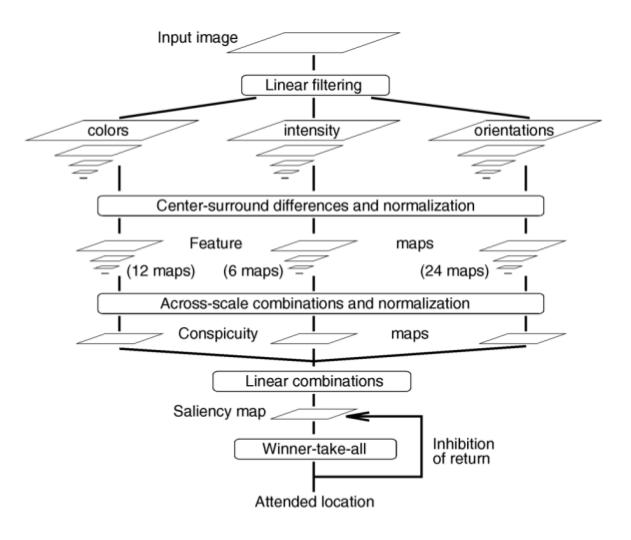
\includegraphics[scale=0.4]{itti_model.jpeg}
	\end{center}
	\caption[Itti-ho hierarchický model vizuálnej pozornosti]{Itti-ho hierarchický model vizuálnej pozornosti\cite{itti}}
\end{figure}

% TODO tiez ako vlastna kapitola
\section{Neurónové siete}
\label{nn}
	 Neurónová sieť je abstraktný výpočtovový model založený na princípe reálnych biologických neurosystémov. Základnou stavebnou jednotkou je tak rovnako ako u neurónových sietí živočíchov neurón, resp. model neurónu\cite{neuron}. Ten spracováva rôzne množstvo vstupov (N) a výstupov (M). V minulosti sa zvykol vyjadrovať podľa nasledovnej matematickej špecifikácie: 
	\begin{equation}
		o_i ^{k+1} = f\left ( \sum_{j+1}^{N} w_{ij}^{k} * o_j^k - \theta_i^{k+1}  \right )
	\end{equation}
	
	Pre vyššie uvedené platí: 
	\newline
	0 \textless i ≤ M
	\newline
	0 \textless j ≤ N
	\newline
	\(o_i^{k+1}\)  - výstupná hodnota i-teho neurónu patriaceho k+1 vrstve 
	\newline
	k - číslo vrstvy
	\newline
	\(\theta_{ij}^{k}\) - prah stimulácie i-teho neurónu k+1 vrstvy
	\newline
	\(w_{ij}^{k}\) - váha medzi i-tym neurónom vrstvy k+1 a j-tym neurónom vrstvy k 
	\newline 
	f() - funkcia
	\newline
	
	V súčasnosti sa však používa radšej matematické vyjadrenie zobrazené v rovnici \ref{eq:new_neuron}. Vypustil sa z neho prah stimulácie neurónu, miesto ktorého sa používa tzv. predsudok (z angl. bias), čo je niečo ako predpokladaná hodnota (náš chýbajúci prah stimulácie) neurónu. Tá sa časom samozrejme mení. 
	
	Predpokladajme, že máme \textit{m+1} vstupov so signálmi od \(x_0\) po \(x_m\) a váhami od \(w_0\) po \(w_m\). Obvykle sa vstupu \(x_0\) pridelí hodnota +1, čím sa stane predsudkom vstupu s \(w_{k0} = b_k\). To necháva potom iba \textit{m} vstupov do neurónu, od \(x_1\) do \(x_m\). Samotný výstup z k-teho neurónu je potom matematicky vyjadrený nasledujúcou rovnicou:
	
	\begin{equation}
		\label{eq:new_neuron}
		y_k = \phi (\sum_{j=0}^{m} w_{kj}*x_j)
	\end{equation}
	
	Pre vyššie uvedené platí:
	\newline
	\(y_k\) - výstup k-teho neurónu
	\newline
	\(w_{kj}\) - váha j-teho neurónu spojeného s k-tym neurónom na ďalšej vrstve
	\newline
	\(x_j\) - j-ty neurón 
	\newline
	\(\phi\) - funkcia
	\newline
	
Neurónová sieť sa sa môže skladať z viacerých vrstiev, na ktorých sú umiestnené neuróny. Prvá vrstva sa nazýva vstupná, posledná výstupná. Medzi nimi môže byť ľubovoľný počet skrytých vrstiev rôzneho typu. Každá vrstva (s výnimkou výstupnej) by mala ešte navyše obsahovať aktivačnú funkciu (kapitola \ref{activation_functions}). V našom prípade sa jedná o neurón umelý a funkciu, ktorá definuje výstup neurónu pre vstup alebo sadu vstupov.
	
\subsection{Aktivačné funkcie}\label{activation_functions}

Aktivačná funkcia predstavuje matematické vyjadrenie použité k aproximácii vplyvu na neurón, zjednušene by bolo možné povedať, že pre sériu vstupov definuje výstupy. Aktivačných funkcií existuje niekoľko typov, každá vhodná na iný typ úloh. Ako príklad je možné uviesť nasledujúce: 
	\begin{itemize}
		\item {\textbf{Softmax}}
		
		Funkcia softmax\footnote{http://eli.thegreenplace.net/2016/the-softmax-function-and-its-derivative/} (inak aj normalizovaná exponenciálna funkcia) normalizuje daný  \textit{n} dimenzionálny vektor tak, že upraví jeho hodnoty do rozsahu (0,1), pričom ich súčet bude rovný 1. Jej matimatické vyjadrenie je nižšie. 
		\begin{equation}
		S_{vec_j} = \frac{e^{vec_j}}{\sum_{i=1}^{n}e^{vec_i}}
		\end{equation}
		
		Pre vyššie uvedené vyjadrenie platí:
		
		\(\forall{\ j\ }\in\ 1..n\)
		
		\(vec \) - konkrétny vector
		
		Keď si ako príklad vezmeme jednoduchý vektor [1, 2, 3], výsledok po aplikovaní softmaxu bude [0.09, 0.24, 0.67]. Ako môžeme vidieť, funkcia sa väčšinou používa na zvýraznenie väčších hodnôt a zárove\ potlačenie hodnôt, ktoré sú výrazne menšie ako maximálna hodnota. 
		
		\item {\textbf{ReLU}}
		
		Upravená lineárna jednotka (z angl. rectified linear unit) je funkcia 
		v tvare:
		\begin{equation}
		f(x) = max (0, x)
		\end{equation}
		kde \textit{x} je vstup do neurónu. Používa sa vďaka svojej jednoduchosti, keďže neobsahuje žiadne komplikované výpočty, čoho dôsledkom je aj jej značná rýchlosť. Jej využitie je možné pozorovať napríklad pri hlbokých neurónových sieťach.
		
		\item{\textbf{Softplus}}
		
		Je v podstate aproximáciou k predošlej ReLU s matematickým vyjadrením:
		\begin{equation}
		f(x)=ln (1 + e^x)
		\end{equation}
		Rovnako ako pri ReLU je oborom hodnôt interval (0, \(\infty\)). Jej využitie je napríklad pri rozoznávaní reči.
		
		\item{\textbf{Sigmoid}}
		
		Táto funkcia sa používa hlavne keď je potrebné pracovať s pravdepodobnosťami, keďže jej výstup tvorí interval (0, 1). Jej matematické vyjadrenie je nasledovné:
		\begin{equation}
		S(t) = \frac{t}{1-e^{-t}}
		\end{equation}
		
		\item {\textbf{Tanh}}
		
		Hyberbolický tangens. Často sa používa v rovnakých prípadoch ako Sigmoid, keďže matematicky sa dá vyjadriť aj za použitia Sigmoidu. Jeho vzorec je nasledovný:
		\begin{equation}
			tanh(x)=\frac{cosh(x)}{sinh(x)}=Sigmoid(2x)-Sigmoid(-2x)=\frac{e^{2x}-1}{e^{2x}+1}
		\end{equation}
	\end{itemize}
	
\subsection{Učenie sa neurónovej siete}
	
Základným prvkom toho, aby bola neurónová sieť schopná riešiť úlohy je učenie sa. Existujú viaceré typy učenia sa neurónovej siete, za zmienku stojí napríklad učenie sa s učiteľom (z angl. supervised learning) a učenie sa bez učiteľa (z angl. unsupervised learning\cite{unsupervised}). Hlavným rozdielom medzi nimi je, že učenie s učiteľom musí prebiehať na predpripravenom datasete, ktorý musí obsahovať nejaké testovacie vstupné dáta (pre ktoré chceme vypočítať výstupnú funkciu) a takzvané štítky (z angl. labels), ktoré sú v podstate naše očakaváne výstupy. Učenie sa bez učeiteľa naproti tomu odvodzuje funkciu k popisu skrytej štruktúry z neoštítkovaných dát, teda bez štítkov, ktoré nám určujú očakaváne výstupy. Nie je tu teda žiadna chyba ani signál k ohodnoteniu potenciálneho riešenia. 
	
	
Príkladom učenia s učiteľom môže byť napríklad jednoduchá neurónová sieť, ktorá má riešiť funkciu XOR\cite{neuron}, kedy potrebujeme reprezentovať vstupné dáta ako dvojicu núl a jednotiek. Štítkami sú v tomto prípade očakávané výstupy, takže napríklad pre vstup (dvojicu) [0,1] je štítkom 1. Takto pripravený dataset pre učenie sa by mal byť veľmi rozsiahly aby sa dosiahla maximálna presnosť. Ďalej je potrebné použiť niektorý z algoritmov učenia. Široko používaným je na takýto typ úloh algoritmus učenia spätného šírenia (z angl. backpropagation). Tento algoritmus sa snaží minimalizovať chybu pri učení a to tak, že najprv sa vypočíta chyba na poslednej (výstupnej) vrstve. Tá sa potom šíri späť k vstupnej vrstve a aktualizujú sa váhy jednotlivých neurónov.  V kombinácii s algoritmami učenia sa používajú optimizačné algoritmy, ktorých cieľom je nájdenie minima funkcie medzi váhami. Medzi základné optimizéry patria:

\begin{itemize}
	\item \textbf{Gradient descent optimizer \cite{gradient_descent}:}
	
	Je to iteratívny algoritmus používaný k nájdeniu lokálneho minima funkcie, kedy podniká kroky k nájdeniu záporného gradientu\footnote{ zmena veličiny v závislosti od inej premennej} funkcie v aktuálnom bode. To je využívané pri určovaní rýchlosti učenia sa neurónovej siete. 
	
	Existujú 3 hlavné varianty gradient descent optimizéru, ktoré počítajú sklon (gradient) funkcie. Delia sa hlavne podľa množstva dát určenému k spracovaniu, kedy sa robí kompromis medzi presnosťou aktualizácie parametra a časom, ktorý je potrebný na vykonanie tejto aktualizácie. Týmito typmi sú:
	\begin{itemize}
		\item{Dávkový gradient descent:}
		
		Z angl. Batch gradient descent. Gradient sa počíta pre celý tréningový dataset, takže pre jednu aktualizáciu je potrebné ho prejsť celý a preto môže byť veľmi pomalý. 
		\item {Stochaistický gradient descent:}
		
		Tento typ je presným kontrastom voči dávkovému gradient descentu. Aktualizácia sa uskutočňuje pre každú vzorku z tréningového datasetu. 
		\item{Mini-dávkový gradient descent:}
		
		Je kompromisom medzi predošlými dvomi typmi. Aktualizácia prebieha pre malú dávku (batch) z datasetu o veľkosti \textit{n} vzoriek.
	\end{itemize} 
	\item \textbf{Adam optimizer \cite{adam}:}
	
	V podstate vychádza priamo zo Stochaistického gradient descent optimizéru, resp. jeho modifikácie RMSProp algoritmu\cite{rms}. Rozdiel oproti Gradient descent optimizéru je ale v tom, že je schopný variabilne určovať rýchlosť učenia neurónovej siete.
	
	\item \textbf{Ftrl optimizer:}
	
	Vychádza z algoritmu učenia FTRL-Proximal\cite{ftrl}, celým názvom Nasleduj regularizovaného vodcu (z angl. Follow The (Proximal) Regularized Leader). Tento algoritmus je bez regularizácie v podstate identický s gradient descentom, avšak používa alternatívnu reprezentáciu koeficientov váh a tak môže byť regularizácia implementovaná efektívnejšie.
\end{itemize}

Po fáze učenia sa nasleduje validácia, pri ktorej sieť nemá prístup k štítkom. Na záver sa prejde k samotnému testovaniu neurónovej siete, kedy sa do nej posúvajú dáta rovnako bez toho, aby sieť mala prístup k štítkom. Na základe jej predikcie a štítkom k testovacím dátam sa určí jej presnosť. Na učenie, testovanie a validáciu by nemali byť použité tie isté dáta. Pomer dát k jednotlivým fázam by mal byť 80-10-10\cite{80-10-10}, čiže 80\% dát je určených na učenie sa, 10\% na validáciu a 10\% na samotné otestovanie predikcií modelu siete. 

Aj keď neurónové siete dokážu efektívne riešiť veľké množstvo úloh, problémom stále zostáva mať k dispozícii dostatok dát k učeniu neurónovej siete ešte pred riešením úloh. Taktiež je potrebné mať dostatok výpočtovej sily, aby sa problém neriešil pridlhý čas, a dostatok pamäte, keďže neurónové siete jej potrebujú značné množstvo. 	
	 
	
\subsection{Typy neurónových sietí}

	Neurónové siete majú niekoľko typov, ktoré  sa rozlišujú hlavne podľa spôsobu prepojenia neurónov, ale aj podľa typu úloh, na ktoré sú určené, či podľa počtu vrstiev neurónov alebo štýlu učenia. %doplnit zdroj
	
	
	Najjednoduchší typ možno zobraziť ako jednu vstupnú vrstvu, jednu skrytú a jednu výstupnú, neuróny sú tu poprepájané z n-tej vrstvy do n+1 vrstvy, ako je možné vidieť na obrázku \ref{simple_nn}. Tento typ sa nazýva dopredná neurónová sieť (z angl. feedforward neural network) a môže mať aj viac ako len jednu skrytú vrstvu. Používa sa hlavne ak sa jedná  o predikciu nelineárnej funkcie (napríklad carbon-13 NMR chemické posuny alkánov\cite{feedforward}). 
	\begin{figure}[H]
		\begin{center}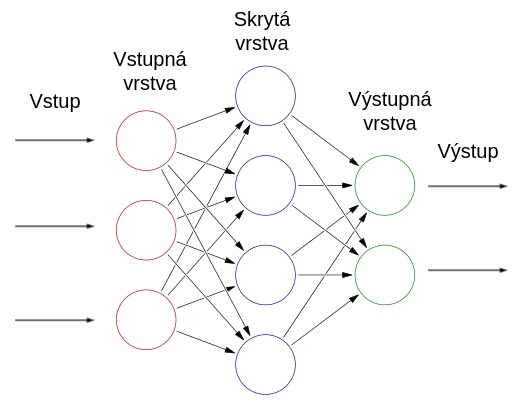
\includegraphics[scale=0.45]{simple_nn.jpg}\end{center}
		\caption[Jednoduchá neurónová sieť]{Príklad jednoduchej neurónovej siete}\label{simple_nn}
	\end{figure}
	
	Zložitejším typom sú rekurentné neurónové siete. Už z názvu vyplýva, že jednou z vecí, ktoré umožňujú, je rekurenciu. Vďaka nej prepojenia neurónov už nie sú jednosmerné len z jednej vrstvy na druhú, ale umožňuje prepojiť neuróny akokoľvek a tak vytvárať napríklad slučky či cykly. To dovoľuje zachytiť aj dynamické časovo obmedzené správanie a používať kontext z minulosti (avšak len niekoľko krokov dozadu), teda použiť niečo ako krátkodobú „pamäť“. Na rozdiel od doprednej neurónovej siete je možné spracovať aj ľubovoľnú sekvenciu vstupov. V praxi to znamená, že keď chceme napríklad predikovať ďalšie slovo vo vete, je dobré vedieť, ktoré slová boli pred ním. Tento typ sietí sa používa napríklad pri rozpoznávaní reči\cite{rnn_speech} alebo písma\cite{rnn_handwriting}, či generovaní popisu k obrázkom\cite{image_description}, kedy však funguje v kombinácii s konvolučnou neurónovou sieťou (z angl. convolutional neural network). Tá je použitá na klasifikáciu obrázkov a rozoznávanie objektov, rekurentná sieť je použitá iba na výsledné generovanie jednoduchého popisu. 
	%TODO asi podobne riesenie ako google drawing treba zistit
	%TODO treba dopisat radial base typ
	Konvolučná neurónová sieť je ďalším typom neurónovej siete, ktorá sa používa pri práci s obrázkami (rozpoznávanie objektov, atď.). Podrobnejšie je tento typ popísaný nižšie, nakoľko je to typ, s~ktorým budeme pracovať aj neskôr. 
	
	\subsubsection{Konvolučné neurónové siete}
	\
	\
	\
	\
	\
	Základ tejto siete tvorí vstupná konvolučná vrstva\footnote{http://www.wildml.com/2015/11/understanding-convolutional-neural-networks-for-nlp/} s konvolučným filtrom, ten býva väčšinou malý (3x3, 5x5). Vstup tejto vrstvy musí byť v tvare \textit{m} x \textit{m} x \textit{r}, kde \textit{m} je šírka a výška obrázku, \textit{r} je počet farebných kanálov. Napríklad pre RGB obrázok je r=3 (červená, zelená, modrá). Konvolučným filtrom sa prejde celý obrázok a výstupom z tejto vrstvy je niekoľko filtrov. Tie sa potom spracúvajú v ďalšie vrstve združovania (z angl. pooling layer\cite{cs231n}), ktorá tieto filtre rozvzorkuje. To prebieha nezávisle na každom získanom filtry z konvolučnej vrstvy. Rozvzorkovanie v podstate znamená, že sa zmení veľkosť filtrov použítim operácie MAX. Najbežnejšou formou spomínanej vrstvy je verzia s oknom (filtrom) o veľkosti 2x2 aplikovaným s krokom veľkosti 2. Toto sa dá jednoducho vysvetliť ako prejdenie každého výstupu z konvolučnej vrstvy oknom uvedenej veľkosti postupne po 2 políčkach na šírku aj výšku, pričom z každej štvorice v okne sa získa MAX operáciou maximum, s ktorým sa pracuje ďalej. Na  obrázku\footnote{http://cs231n.github.io/convolutional-networks/} \ref{fig:cnn} je vidieť výsledok popisovaného postupu na jednoduchom príklade.
	
	\begin{figure}[H]
		\begin{center}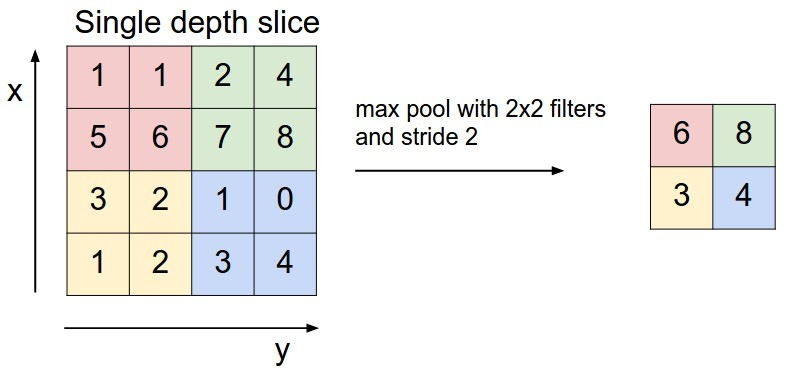
\includegraphics[scale=0.38]{maxpool.jpeg}\end{center}
		\caption[Vrstva združovania - príklad vzorkovania]{Príklad vrstvy združovania, pri ktorom sa rozvzorkuje výstup z konvolučnej vrstvy o veľkosti 4x4, filtrom 2x2, s krokom veľkosti 2 za použitia operácie MAX}\label{fig:cnn}
	\end{figure}
	Takýchto konvolučných vrstiev s vrstvami združovania môže byť aj viac, nemusia ani nutne nasledovať po sebe. Po týchto vrstvách nasleduje plne prepojená vrstva alebo vrstvy (z angl. fully-connected layers), čo je vrstva, v ktorej majú neuróny plné spojenie so všetkými aktiváciami v predošlej vrstve, rovnako ako pri bežných neurónových sieťach. Aktivačnou funkciou neurónov na tejto vrstve býva väčšinou ReLU. Po plne prepojenej vrstve (vrstvách) už nasleduje iba výstupná vrstva. Na obrázku\footnote{https://ujjwalkarn.me/2016/08/11/intuitive-explanation-convnets/} nižšie je jednoduchý náčrt vyššie popísané konvolučnej neurónovej siete. 
	\begin{figure}[H]
		\begin{center}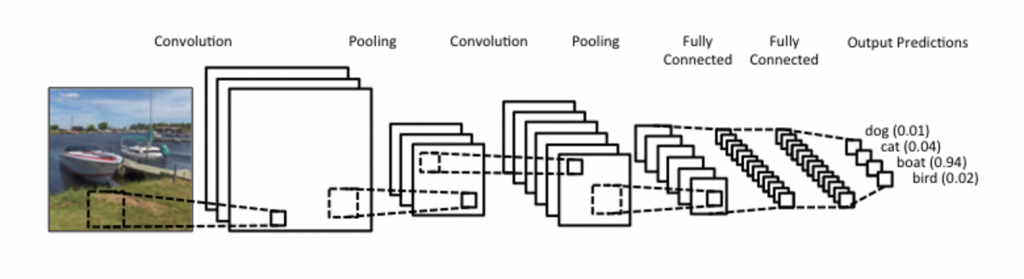
\includegraphics[scale=0.38]{cnn.png}\end{center}
		\caption[Konvolučná neurónová sieť]{Príklad konvolučnej neurónovej siete}\label{conv_nn}
	\end{figure}
	
	Využite tohto typu je v podstate všade, kde sa jedná o rozpoznávanie obrázkov. Či už ide o automatické vyznačenie tvárí pre označenie na facebooku, autonómne vozidlá, ktoré sa vedia riadiť sami (autopilot) alebo triedenie uhoriek na farmách v Japonsku\footnote{https://cloud.google.com/blog/big-data/2016/08/how-a-japanese-cucumber-farmer-is-using-deep-learning-and-tensorflow}. Na tento konkrétny softvér bol použitý príklad kódu jednoduchej konvolučnej siete z tutoriálu\footnote{https://www.tensorflow.org/versions/0.6.0/tutorials/mnist/pros/index.html} pre TensorFlow (knižnica pre prácu s neurónovými sieťami), s modifikáciou konvolučnej a združovacej vrstvy tak, aby bola sieť uspôsobená počtu tried uhoriek (10) a ich formátu obrázkov. 
	
	
	Z mnohých pokusov o autonómnu jazdu stoja za zmienku hlavne tie od Tesly a Google. Prototyp autonómneho systému vozidla od Google-u Dave-2\cite{google_car} využíva model neurónovej siete s 9 vrstvami, jednu normalizačnú, 5 konvolučných a 3 plne prepojené vrstvy. Kamerami spracovaný obraz okolia s frekvenciou 10 snímkov za sekundu (tak nízky počet preto, aby sa predišlo veľkému množstvu príliš podobných obrázkov) je po jednom snímku rozdelený do YUV\footnote{farebný priestor používaný vo video aplikáciách} úrovní a posunutý do neurónovej siete.   
 
\subsection{Framework-y pre prácu s neurónovými sieťami}
V dnešnej dobe moderného internetu a dostupnosti technológií máme možnosť výberu z dostatočného množstva framework-ov pre potreby riešenia najrôznejších problémov neurónovými sieťami. Pri výbere môžeme brať do úvahy napríklad preferencie operačného systému (Windows, Linux, ...), programovacieho jazyka (Python, C++, Java, ...), ale aj benefity distribuovaného riešenia a omnoho viac. V nasledujúcich podkapitolách sú preto popísané niektoré z najpoužívanejších technológií pre implementovanie neurónových sietí. 

%TODO mozno prihodit ukazky zdrojakov
\subsubsection{TensorFlow}
TensorFlow\footnote{https://www.tensorflow.org/} je open-source softvérová knižnica, ktorá pre numerické výpočty používa graf dátového toku, kde uzly grafu reprezentujú matematické operácie a hrany multidimenzionálne dátové polia, tzv. tenzory. Graf je možné skonštruovať použitím jazykov s podporou frontend-u (C++, Python, ...). 

Flexibilná architektúra umožňuje vykonávať výpočty na CPU alebo GPU (nepomerne rýchlejšie) na serveroch, desktopových počítačoch či dokonca aj mobilných zariadeniach. Pôvodne bol TensorFlow vyvinutý výzkumníkmi a inžiniermi v Google-i pre strojové učenie a hlboké učenie, avšak jeho využitie je oveľa širšie. Momentálne používa TensorFlow veľké množstvo programov, napríklad Google vyhľadávač, prekladač alebo YouTube. 

Momentálne podporuje jazyky C++, Python, Java, Go, Swift.

Medzi hlavné výhody patrí:
\begin{itemize}
	\item podpora pre jednoducho naučiteľné jazyky (Python)
	\item použtie výpočtovej grafovej abstrakcie
	\item vizualizácie pomocou TensorBoard-u\footnote{https://www.tensorflow.org/programmers\_guide/summaries\_and\_tensorboard} (interaktívne grafy pre priebeh učenia, pre model siete, ...)
	\item dostatočne nízko-úrovňový pre plnú kontrolu a implementáciu vlastnej (novej nie len preddefinovanej) funkcionality (v porovnaní napríklad s framework-om Keras(kapitola \ref{keras}))
\end{itemize}

Ako nevýhody možno uviesť:
\begin{itemize}
	\item nedostatok predtrénovaných modelov
	\item pri použití s určitými jazykmi (Python, Java, ...) je pomalý, nakoľko sa nejedná najrýchlejšie jazyky
\end{itemize}

\subsubsection{Microsoft CNTK}
Označuje knižnicu Microsoft Cognitive Toolkit\footnote{https://docs.microsoft.com/en-us/cognitive-toolkit/}, ktorá zlepšuje modularizáciu a údržbu separácie výpočtových sietí, zároveň postkytuje algoritmy učenia a popisy modelov. Má sa jednať o odpoveď na TensorFlow, poskytovaná funkcionalita je veľmi podobná, avšak je o niečo rýchlejší. Princíp a celá architektúra sú zachytené na diagrame na obrázku \ref{cntk_image}. 

\begin{figure}[H]
	\begin{center}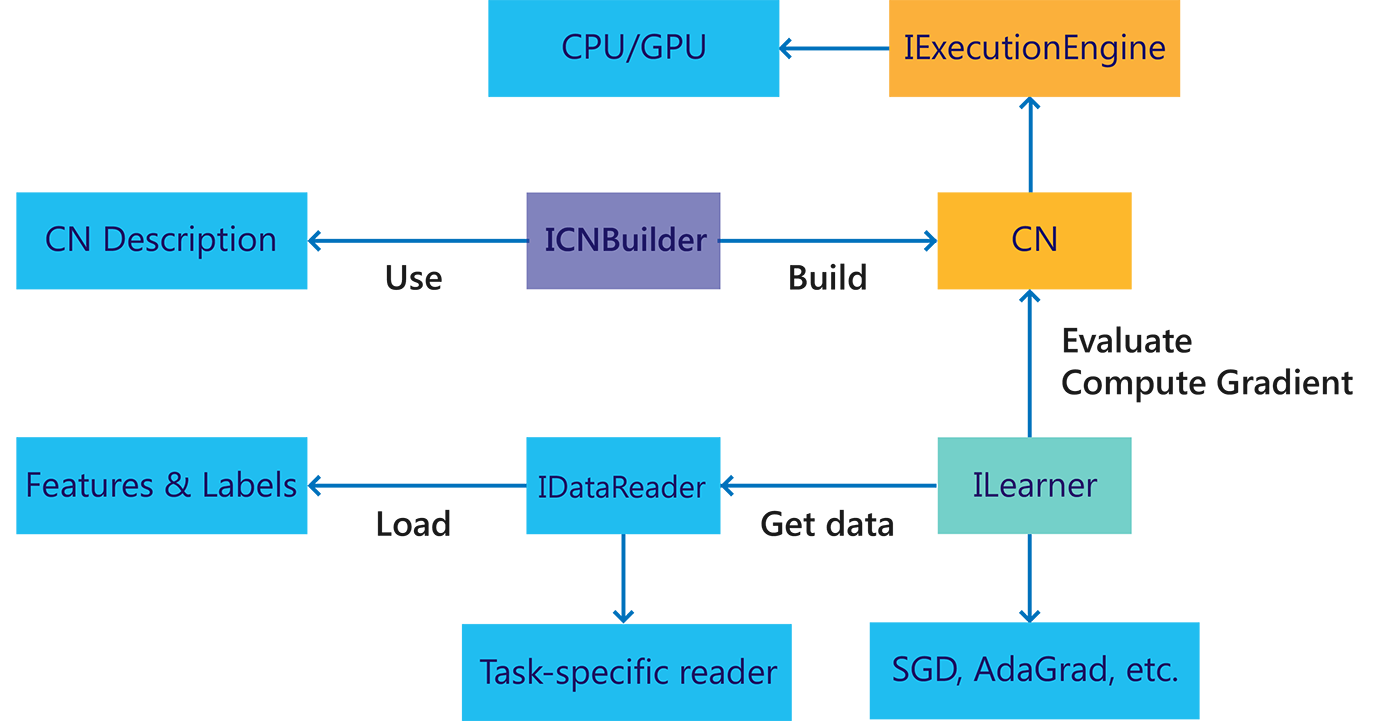
\includegraphics[scale=0.3]{microsoft-cntk-architecture.png}
		\caption[Architektúra fungovania Microsoft CNTK]{
			Diagram zobrazujúci architektúru fungovania Microsoft CNTK\footnotemark
		}\label{cntk_image}
	\end{center}
\end{figure}
\footnotetext{https://dzone.com/articles/progressive-tools10-best-frameworks-and-libraries}

Momentálne podporuje jazyky C++, C\#, Python, Java.

Výhodami tohto framework-u sú:
\begin{itemize}
	\item flexibilita
	\item umožňuje distribuovaný tréning
\end{itemize}

Medzi nevýhody možno zaradiť:
\begin{itemize}
	\item implementácia v novom jazyku, Network Description Language (NDL)
	\item nedostatok možností a nástrojov pre vizualizácie
\end{itemize}

\subsubsection{Theano}

Theano\footnote{https://github.com/Theano/Theano} je veľmi silná knižnica umožňujúca definovanie, optimalizáciu a evaluáciu numerických operácií nad multidimenzionálnymi poliami s obrovskou efektivitou. Podobne ako TensorFlow, k abstrakcii výpočtov používa grafy, ako možno vidieť na príklade na obrázku \ref{theano_image}.

% theano-data-visualization.png

\begin{figure}[H]
	\begin{center}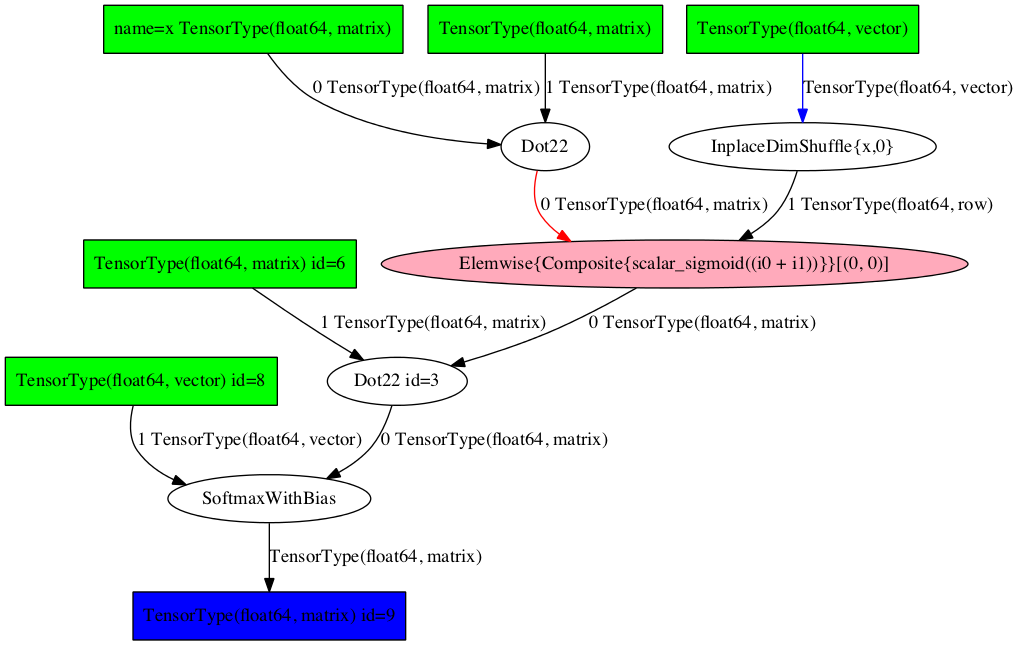
\includegraphics[scale=0.4]{theano-data-visualization.png}
		\caption[Príklad grafovej abstrakcie výpočtov použitím framework-u Theano]{
			Príklad grafovej abstrakcie výpočtov použitím framework-u Theano\footnotemark
		}\label{theano_image}
	\end{center}
\end{figure}
\footnotetext{http://www.wildml.com/2015/09/speeding-up-your-neural-network-with-theano-and-the-gpu/}

Momentálne podporuje iba programovací jazyk Python a v poslednej dobe vývoj tohto framework-u dosť upadá.

Medzi hlavné výhody patrí:
\begin{itemize}
	\item veľmi dobrá optimalizácia pre CPU a GPU (najmä vďaka použitiu nízko-úrovňovej funkcionality naprogramovanie v jazyku C)
	\item vysoko efektívna knižnica pre numerické úlohy
\end{itemize}

Za najväčšie nevýhody sú pokladané:
\begin{itemize}
	\item Theano samo o sebe je v porovnaní s ostatnými knižnicami príliš nízko-úrovňové
	\item potreba použitia s inými knižnicami s vyšším stupňom abstrakcie (napríklad Keras) 
\end{itemize}

\subsubsection{Keras}\label{keras}

\subsubsection{Spark MLlib}

\section{Existujúce riešenia}

\section{Metriky používané na ohodnotenie modelov vizuálnej pozornosti}
\label{metric}
Tradične sa tieto modely evaluujú vzhľadom na pohyb očí, resp. samotné fixácie. K tomu slúži značný počet rôzne fungujúcich metrík\cite{metriky}, najpoužívanejšie sú:

\begin{itemize}
	
	\item NSS - Normalizovaná cesta pútavosti (z angl. Normalized Scanpath Saliency). Využíva priemer hodnôt pútavosti na \textit{n} fixácií v normalizovanej mape podľa nasledovného vzorca: 
	
	\begin{equation}
	\frac{1}{n} \sum_{i=1}^{n} \frac{s(x_{h}^{i}, y_{h}^{i}) - \mu_{s}}{\sigma _{s}}
	\end{equation}
	
	\item AUC - Oblasť pod ROC krivkou (z angl. Area Under the ROC Curve).
	Ľudské fixácie sú považované za pozitívnu sadu a niektoré body na obrázku sú vybrané ako negatívna sada. K mape pútavosti je potom pristupované ako k binárnemu klasifikátoru na separáciu pozitívnych vzorkov od negatívnych. Presnosť podľa tejto metriky je daná nasledovne: 
	
	\begin{itemize}
		
		\item 0.90 - 1 = výborná
		\item 0.80 - 0.90 = dobrá
		\item 0.70 - 0.80 = priemerná
		\item 0.60 - 0.70 = slabá
		\item 0.50 - 0.60 = veľmi slabá
		
	\end{itemize}
	
	\item sAUC - Zamiešaná oblasť pod ROC krivkou (z angl. shuffled Area Under the ROC Curve) je mierna modifikácia vyššie uvedenej metriky, kedy ako negatívna sada nie sú vybrané len niektoré body, ale všetky body, ktoré nie sú ľudskými fixáciami, sú považované za negatívne. Určenie presnosti na základe hodnôt je rovnaké ako pri AUC. 
	
	\item CC - Korelačný koeficient, určuje prakticky podobnosť v tomto prípade dvoch máp výraznosti, kde jedna je výsledok modelu vizuálnej pozornosti a druhá je reálna mapa vypočítaná z fixácií. 
	
	\begin{equation}
	CC (s, h) = \frac{cov(s, h)}{\sigma_{s} \sigma _{h}}
	\end{equation}
\end{itemize}
 
 
% ----------------------------------------------------------------------------------------
\iffalse	
\subsection{Určenie pútavých častí webových stránok pomocou strojového učenia}
\label{machine_learning}
	V nasledujúcej časti sú opísané niektoré z existujúcich riešení problému určenia pútavých častí grafického rozhrania webovej stránky za použitia strojového učenia. V podstate existujú 2 prístupy, z ktorých jeden vychádza z HTML kódu stránku a druhý len z jej obrázku, screenshot-u. 
	

\subsubsection{Riešenia na báze segmentácie stránok}

	Tento spôsob na začiatku vyhádza z HTML kódu stránky, ktorú na jeho základe rozdelí tzv. segmentovaním na hlavné časti (segmenty, bloky) stránky. Segmentácia používa buď segmentačné algoritmy na rozdelenie stránky do blokov podľa rôznych vlastností, alebo používa dátové štruktúry na reprezentáciu komponentov a elementov HTML dokumentu. 
    Najpoužívanejšie prístupy k segmentácii sú:
\begin{my_itemize}
	\item {Segmentácia založená na DOM\cite{DOM} (dokumentový objektový model, z angl. document object model):}
	\newline
\hspace{10mm}HTML dokument je reprezentovaný ako DOM strom. Tagy môžu reprezentovať jeden blok stránky, napr. P-paragraf, TABLE-tabulka, atď. I keď tento strom dokáže veľmi presne reprezentovať štruktúru HTML dokumentu (stránky), často nie je dostatočne presný pri 	rozdelení sémanticky (vizuálne) rôznych blokov. 
	\item {Segmentácia založená na lokácii\cite{block_importance} (z angl. location-based segmentation):}
	\newline
\hspace{10mm}Stránka sa rozdelí na 5 hlavných častí: stred, vľavo, vpravo, hore, dolu. Problémom je však, že nie vždy sa toto rozdelenie hodí na každú stránku a v prípade, že je stránka príliš dlhá (scroll-ovateľná) sa časti, ktoré boli na začiatku napr. dolu, posunú smerom hore a rozdelenie stránky sa tým zmení. 
	\item {VIPS\cite{vips} - segmentácia stránky založená na pohľade (z angl. vision-based page segmentation):}
	\newline
\hspace{10mm}VIPS je v podstate kombinácia predchádzajúcich dvoch algoritmov. Delí stránku aj na základe farby, veľkosti blokov atď. V prvom rade vyberie vhodné uzly z DOM stromu a nájde medzi nimi separátory, ktoré naznačujú horizontálne a vertikálne línie webovej stránky. Na základe DOM stromu a separátorov sa vytvorí sémantický strom stránky, v ktorom je každý segment stránky reprezentovaný ako samostatný uzol v strome, koreňom stromu je samotná stránka. Spojitosť segmentácie stránky je kontrolovaná prededifinovaným stupňom koherencie ( z angl. Predefined Degree of Coherence (PDoC\cite{PDOC})) – každému uzlu je daný určitý stupeň súvislosti, čo zabezpečuje, že VIPS dokáže efektívne držať obsah pokope, zatiaľ čo sémanticky odlišné bloky od seba.
\end{my_itemize}

	Ako príklad riešenia používajúceho spomínanú segmentáciu je možné uviesť prácu výskumníkov z Microsoftu \cite{block_importance}. Tí použili VIPS algoritmus na segmentovanie a 5 ľudí, ktorí manuálne oštítkovali každý blok webovej stránky. Bloky sú očíslované od 1 po 4 podľa dôležitosti (1 – nepodstatné informácie ako reklamy, 4 – najdôležitejšia časť stránky, hlavný obsah). Z nich sa potom zostrojí model dôležitosti blokov, čo je vlastne funkcia mapovania každého bloku a jeho dôležitosti zobrazená ako:    
	\begin {center}
	\center \{ block features \} → block importance
	\newline
	\end {center}

	Vizualizácia mapovania dôležitosti blokov je zobrazená na časti stránky na obrázku \ref{fig:cnn_rbf}.

		\begin{figure}[H]
			\begin{center}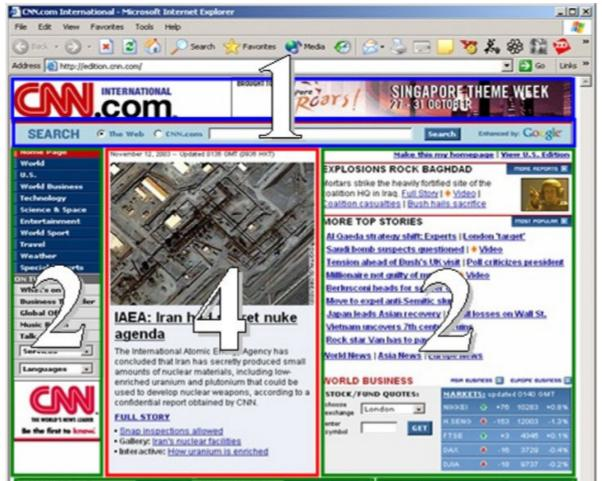
\includegraphics[scale=0.3]{cnn_rbf.jpeg}\end{center}
			\caption[Vizualizácia mapovania dôležitosti blokov webových stránok]{Vizualizácia mapovania dôležitosti blokov webových stránok\cite{block_importance}. 1 - najmenej dôležité informácie, 4 - najpodstatnejšia časť stránky}\label{fig:cnn_rbf}
		\end{figure}

	Na odhad dôležitosti blokov sa potom nahliada ako na regresný problém a na jeho riešenie je  použitá neurónová sieť, v ktorej sú bloky reprezentované ako dvojica (\textit{x, y}), kde \textit{x} je reprezentácia bloku a \textit{y} je dôležitosť (berie sa ako reálne číslo).  Typ siete je RBF (radial basis function) a vyhľadávacou technikou je štandardný gradient descent. Sieť zahŕňa 3 vrstvy, každú s inou funkciou. Prvú (vstupnú) vrstvu tvoria zdrojové uzly, druhá je jediná skrytá vrstva a zabezpečuje nonlineárnu transformáciu zo vstupného priestoru do skrytého. Obsahuje RBF neuróny, ktoré kalkulujú vstup skrytej vrstvy kombináciou vážených vstupov a odhadov. Tretia (výstupná) vrstva dodáva dôležitosť blokov do reprezentácie blokov aplikovanej v prvej (vstupnej) vrstve. 
	
	Výhodou tohto riešenia je rozdelenie stránky podľa logických blokov, nevýhodu vidím v začiatočnom ohodnotení blokov ľuďmi podľa dôležitosti, pretože mi to príde príliš individuálne. Tiež rozdelenie stránky do stromu s jednotlivými blokmi a časťami je v závislosti od stránky dosť pamäťovo náročná operácia. 
	
\subsubsection{Riešenia vychádzajúce z obrázku stránky}
\label{singapur}
	Tento typ riešenia používa k určeniu dôležitých (pútavých) častí stránky jej screenshot. Autormi modelu sú Chengyao Shen a Qi Zhao\cite{singapur_model}. Tí na začiatku rozdelili ich dataset do niekoľkých kategórií podľa obsahu stránky, t. j. ilustrované (prevládajú obrázky), textové (prevažne blogy, články, atď.) a mix predošlých dvoch kategórií. V každej z nich bolo približne 50 obrázkov s rozlíšením 1360x768. Na obrázky web stránok  potom pozeralo 11 subjektov a ich sekvencie pohľadov boli zaznamenané pomocou MATLABU s Psychtoolbox\cite{psych} a systémom Eyelink 1000.
	
	Na predikciu pohľadov\cite{saliency} na web stránky bola použitá metóda MKL (Multiple Kernel Learning - kombinuje viacero jadier SVM\footnote{Support Vector Machine - modely učenia s príslušnými algoritmami učenia, ktoré analyzujú dáta použité pre klasifikáciu a regresnú analýzu\cite{SVM}} miesto jedného). MKL bolo trénované ako binárny regresný problém, z datasetu bolo použitých 119 obrázkov na trénovanie, zvyšných 30 bolo použitých na finálne testovanie. Predikovaný bol vektor pohľadov (fixácií) na obrázok. Vyhodnotením datasetu bolo zistené, že človeka mimo iné upúta pri pohľade na web stránku v prvom rade ľudská tvár, oči a celkovo horná časť tela, či neprimerane veľké logo. Taktiež sa dá predpovedať, že človek sa začne pozerať v prvom rade najprv do strednej  oblasti a oblasti viac vľavo hore od stredu. Tieto zistenia dokázali veľmi dobre zapracovať aj do ich modelu. Na obrázku nižšie je možné vidieť vizualizáciu pohľadu na rôzne typy stránok v prvých 5 sekundách formou teplotných máp.
		\begin{figure}[H]
			\begin{center}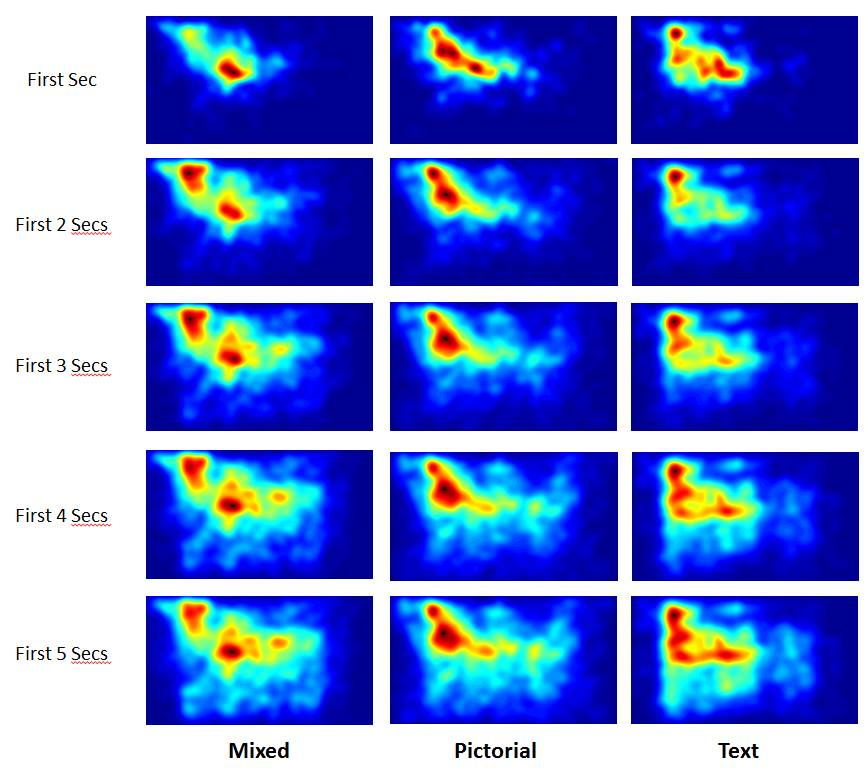
\includegraphics[scale=0.3]{heatmaps.png}\end{center}
			\caption[Vizualizácia pohľadu formou teplotných máp]{Vizualizácia pohľadov v prvých 5 sekundách. Vľavo mix stránok, v strede prevažne ilustrované stránky a vpravo textové.\cite{singapur_model}}%\label{simple_nn}
		\end{figure}
		
	Za výhodu tohto riešenia oproti predošlému pokladám hlavne vygenerovanie heat mapy, ktorá vypovie o dôležitých častiach stránky ďaleko viac ako očíslované HTML bloky. Taktiež zistenia, že človek si ako prvé všíma napríklad ľudské tváre, sú pre dizajnéra web stránky určite velké plus oproti dôležitosti informácií na základe ich umiestnenia. 
\fi